\documentclass[a4paper,USenglish,cleveref,autoref,thm-restate]{lipics-v2021}

\usepackage{tikz-cd}
\usetikzlibrary{arrows.meta,positioning,shapes,calc,decorations.pathreplacing,3d,fit}
\usepackage{siunitx}
\sisetup{group-separator={\,},group-minimum-digits=4}
\usepackage{booktabs}
\usepackage{listings}
\usepackage{microtype}
\emergencystretch=1.5em
\lstset{basicstyle=\ttfamily\small,columns=fullflexible,keepspaces=true,literate={→}{{$\to$}}1 {∀}{{$\forall$}}1 {≤}{{$\le$}}1}

\newcommand{\Len}{\operatorname{Len}}
\newcommand{\word}[1]{\texttt{#1}}
\newcommand{\Z}{\mathbb{Z}}
\newcommand{\R}{\mathbb{R}}
\newcommand{\lean}[1]{\texttt{#1}}
\newcommand{\Kft}{K_{5_2}}
\newcommand{\NWords}{\num{33000}}
\newcommand{\NNodes}{\num{2.27e12}}
\newcommand{\NodeBase}{2.493}
\newcommand{\NodeConst}{5.67\times 10^{-2}}
\newcommand{\NodeRatio}{6.21}
\newcommand{\WordBase}{1.836}
\newcommand{\WordConst}{2.68\times 10^{-5}}
\newcommand{\RatioFirst}{5.1}
\newcommand{\RatioLast}{6.8}

\sisetup{exponent-product=\times,print-unity-mantissa=false}

\bibliographystyle{plainurl}

\title{The Knot $5_2$ Needs 36 Steps on the Cubic Lattice}
\titlerunning{The Knot $5_2$ Needs 36 Steps on the Cubic Lattice}

\author{Author names to be inserted}{Affiliation to be inserted}{}{}{}
\authorrunning{Authors}
\Copyright{}

\ccsdesc[500]{Mathematics of computing~Topology}
\ccsdesc[300]{Theory of computation~Logic and verification}

\keywords{Lattice knots, minimal step number, exhaustive enumeration, Fox colourings, formal verification, Lean}

\supplement{All programs, proofs, logs and certificates: \url{https://github.com/srinjoysom11/-K-NOT_THEORY}, directory \texttt{research/exact}.}

\nolinenumbers
\hideLIPIcs

\begin{document}
\maketitle

\begin{abstract}
A knot drawn as a closed walk on the cubic lattice $\Z^3$ needs a certain least number of unit
steps, its \emph{minimal lattice length}.  This number is known for only three knots: the trefoil
needs 24 steps, the figure-eight knot 30 and the cinquefoil $5_1$ needs 34.  For every other knot only
upper bounds were known.  We prove that the knot $5_2$ needs exactly 36 steps.

The proof has three stages.  (1) A normal form: we show that a shortest $5_2$ polygon can be moved,
by square moves that do not change the knot or the length, into a position where a list of local
conditions holds.  (2) An exhaustive search: a depth-first enumeration of all closed walks of length
at most 34 that satisfy these conditions, pruned only by tests that are theorems about them.
(3) Certificates: every one of the \NWords{} words the search returns has a regular diagram whose
Fox $7$-colourings are all constant, while every diagram of $5_2$ has $49$ of them.

Every step is formalised in the Lean~4 proof assistant: the normal-form theorem, the completeness of
the search program, the soundness of the colouring certificates and the identification of the
36-step example are kernel-checked, with no axioms beyond Lean's standard three.  The
computation itself, \num{1358} closed Boolean terms evaluated by the compiled verified program
(about \NNodes{} search nodes in all), was run on a laptop-sized container and on GitHub's free
runners, and was cross-checked against an independent C\texttt{++} implementation of the same search.
We describe the mathematics, the search, and the engineering that made a proof of this size
checkable.
\end{abstract}

%=====================================================================================================
\section{Introduction}

Take a knot and build it from unit sticks that lie along the edges of the cubic lattice: every stick
runs from one integer point to a neighbouring one, and the sticks close up into a polygon that does
not touch itself.  How few sticks are needed?  This number, the \emph{minimal lattice length}
$\Len(K)$ of the knot type $K$, is one of the simplest measures of how complicated a knot is, and it
has been studied since the 1990s both as a question in geometric knot theory and because lattice
polygons are the standard model of ring polymers in statistical physics~\cite{Diao93,Sch09,JvRR11}.

Upper bounds are easy in principle: exhibit a polygon.  Simulated annealing and other stochastic
searches have produced short polygons for all knots with up to ten crossings, and these are believed
to be optimal for small knots~\cite{Sch09,JvRR11}.  Lower bounds are hard.  Diao proved in
1993 that every non-trivial knot needs at least 24 steps and that the trefoil attains
this~\cite{Diao93}.  Scharein, Ishihara, Arsuaga, Diao, Shimokawa and Vazquez reported that the
figure-eight knot needs 30 steps and the cinquefoil $5_1$ needs 34~\cite{Sch09}.  Beyond these three
knots no exact value was known; for $5_2$, the second knot with five crossings, a 36-step polygon is
known~\cite{Sch09,JvRR11}, but no matching lower bound had been proved.

\begin{theorem}[Main theorem]\label{thm:main}
$\Len(5_2)=36$.
\end{theorem}

\begin{figure}[t]
\centering
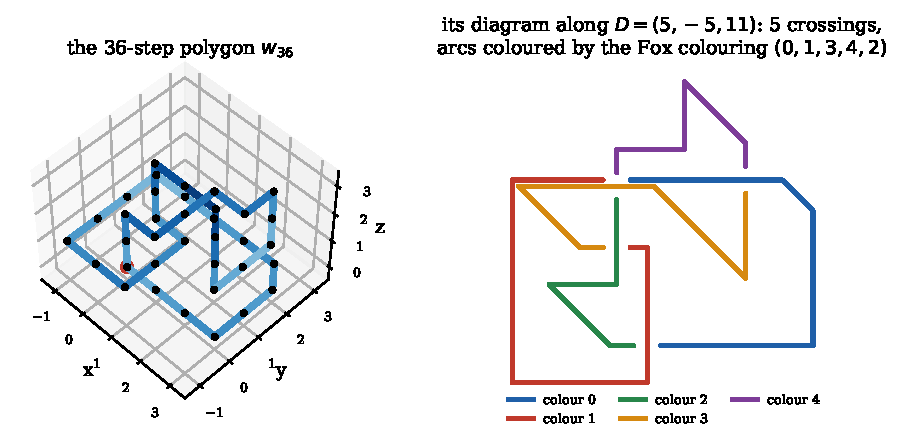
\includegraphics[width=\linewidth]{figs/polygon36.pdf}
\caption{Left: a 36-step lattice polygon of type $5_2$; the red dot is the origin.  Right: its
projection along $(5,-5,11)$ is the standard 5-crossing diagram of $5_2$.  The five arcs are coloured
by a Fox $7$-colouring that is not constant (\cref{sec:colour}); the existence of such a colouring is
what distinguishes $5_2$ from every short polygon the search returns.}
\label{fig:polygon}
\end{figure}

The upper bound is the polygon of \cref{fig:polygon}.  The content of the theorem is the lower bound:
\emph{no lattice polygon with 34 or fewer steps is a $5_2$}.  There are of the order of $10^{18}$ lattice
polygons of length $34$, far too many to enumerate.  Our proof avoids enumerating them by
enumerating only candidates for one carefully chosen shortest representative, and it rules out each
candidate by a short, independently checkable algebraic certificate.  The proof proceeds in three
stages, which we describe in turn.

\begin{enumerate}
\item \textbf{A normal form} (\cref{sec:normal}).  If $5_2$ had a polygon with at most 34 steps,
then a particular one of the shortest such polygons---pushed as far down as possible, in a canonical
position---would satisfy seven local conditions C1--C7.  The conditions come from two kinds of
square moves, which change a polygon without changing its knot type.
\item \textbf{An exhaustive search} (\cref{sec:search}).  A depth-first search lists every closed walk
of length at most 34 that satisfies C1--C7.  It discards a partial walk only when a test shows that
no completion can satisfy them; each test is a theorem.  The search visits about \NNodes{}
partial walks and returns \NWords{} words.
\item \textbf{Certificates} (\cref{sec:colour}).  Each returned word comes with a regular diagram and
a matrix certificate showing that every Fox $7$-colouring of that diagram is constant.  Every
diagram of $5_2$ has non-constant ones, so none of the words is a $5_2$.
\end{enumerate}

This is a computer-assisted proof, and it is natural to ask how much of it one must take on trust.
Our answer is \emph{very little}.  All three stages are formalised in Lean~4~\cite{Lean4}
(\cref{sec:lean}): the normal-form theorem, the completeness of the actual search program that was
run, and the soundness of the certificates are theorems checked by the Lean kernel.  What remains
is (i) a short list of definitions that state the theorem, (ii) two classical facts of knot theory
($\Delta$-moves preserve knot type; the Wirtinger presentation of the knot group), and (iii) the evaluation of
\num{1358} closed Boolean terms by the compiled program, which we cross-checked against an
independent C\texttt{++} implementation that agrees node for node.  In particular, \emph{the pruning
of the search is not trusted}: every discarded branch is discarded by a test that Lean has proved can
never discard a $5_2$.

We stress what is \emph{not} used.  Earlier versions of this search, run to length 36, used two
further lemmas---a plane-crossing lemma valid only for prime knots, and a computer-checked lemma
about short knotted arcs---that made it about five times faster.  They are not part of the proof
presented here; the final search uses only conditions C1--C7, which hold for every knot type.

\paragraph*{Organisation.}  \Cref{sec:prelim} fixes definitions.  \Cref{sec:normal,sec:search,sec:colour}
are the three stages, and \cref{sec:upper} is the upper bound.  \Cref{sec:lean} describes the
formalisation and \cref{sec:engineering} the computation and its engineering; \cref{sec:cross} lists
the independent cross-checks, and \cref{sec:discussion} closes with open problems.

%=====================================================================================================
\section{Preliminaries}\label{sec:prelim}

\paragraph*{Lattice polygons.}  The six unit vectors of $\Z^3$ are written
$\word{e},\word{w},\word{n},\word{s},\word{u},\word{d}$ for $\pm x$, $\pm y$, $\pm z$.  A \emph{word}
$w=w_0w_1\cdots w_{n-1}$ in these letters describes the walk with vertices $v_0=0$ and
$v_{i+1}=v_i+w_i$.  It is a \emph{polygon word} if $n\ge 4$, $v_n=0$ and $v_0,\dots,v_{n-1}$ are
distinct; its \emph{polygon} $|w|$ is the union of the $n$ unit segments $[v_i,v_{i+1}]$, a simple
closed curve.  Every lattice polygon is a translate of $|w|$ for some polygon word.  Polygon words
have even length, since each axis is crossed equally often in both directions.

\paragraph*{Knots.}  Two polygonal knots are equivalent if an orientation-preserving homeomorphism of
$\R^3$ carries one onto the other.  A \emph{$\Delta$-move} replaces an edge $[a,b]$ by $[a,c]\cup[c,b]$ (or
the reverse) when the triangle $abc$ meets the knot only in those edges; $\Delta$-moves do not change the
knot type.  We use knot types without orientation, and write $K^*$ for the mirror image of $K$.
$\Len(K)$ is the least length of a lattice polygon of type $K$; clearly $\Len(K^*)=\Len(K)$.

\paragraph*{Diagrams and colourings.}  A linear projection of a knot to the plane is \emph{regular}
if it has finitely many multiple points, all transverse double points, none of them the image of a
vertex.  The over-strand at each crossing is the one nearer the viewer.  Cutting the image at every
under-passage gives the \emph{arcs} of the diagram.  A \emph{Fox $p$-colouring}~\cite{Fox62,Prz98}
assigns to each arc an element of $\Z/p$ so that at every crossing
\[ 2\cdot(\text{over-arc}) \equiv (\text{incoming under-arc}) + (\text{outgoing under-arc}) \pmod p. \]
Constant assignments are always colourings.  For $p=7$ the standard diagram of $5_2$ has $49$
colourings (\cref{lem:fiftytwo}), while the unknot, the trefoil, the figure-eight knot and $5_1$ have
only the $7$ constant ones; this is the invariant we use.

%=====================================================================================================
\section{Stage one: a normal form for a shortest polygon}\label{sec:normal}

Suppose some polygon of type $5_2$ or $5_2^*$ has at most 34 steps, and let $m$ be the least length
of such a polygon.  We now choose one shortest polygon very carefully, and show that the choice forces
seven local conditions.  The tools are two moves across a unit square.

\begin{figure}[t]
\centering
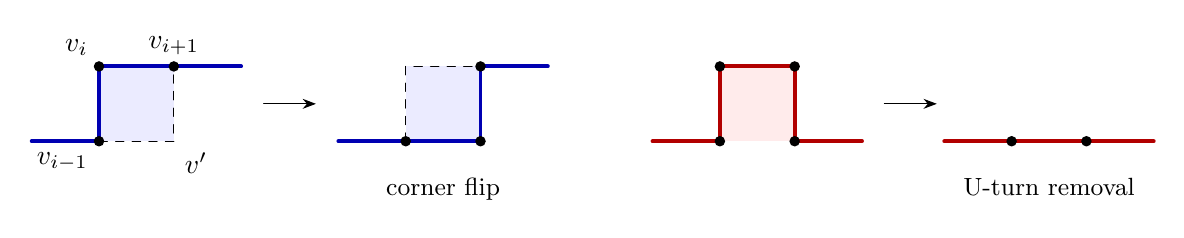
\begin{tikzpicture}[scale=0.95,line width=1.4pt,line cap=round]
\begin{scope}
  \fill[blue!8] (0,0) rectangle (1,1);
  \draw[blue!70!black] (-0.9,0) -- (0,0) -- (0,1) -- (1,1) -- (1.9,1);
  \foreach \p in {(0,0),(0,1),(1,1)} \fill \p circle (2pt);
  \draw[dashed,thin] (0,0) -- (1,0) -- (1,1);
  \node[below left] at (0,0) {$v_{i-1}$}; \node[above left] at (0,1) {$v_i$};
  \node[above] at (1,1) {$v_{i+1}$}; \node[below right] at (1,0) {$v'$};
  \draw[-{Stealth},thin] (2.2,0.5) -- (2.9,0.5);
\end{scope}
\begin{scope}[xshift=4.1cm]
  \fill[blue!8] (0,0) rectangle (1,1);
  \draw[blue!70!black] (-0.9,0) -- (0,0) -- (1,0) -- (1,1) -- (1.9,1);
  \foreach \p in {(0,0),(1,0),(1,1)} \fill \p circle (2pt);
  \draw[dashed,thin] (0,0) -- (0,1) -- (1,1);
  \node[below] at (0.5,-0.35) {\small corner flip};
\end{scope}
\begin{scope}[xshift=8.3cm]
  \fill[red!8] (0,0) rectangle (1,1);
  \draw[red!70!black] (-0.9,0) -- (0,0) -- (0,1) -- (1,1) -- (1,0) -- (1.9,0);
  \foreach \p in {(0,0),(0,1),(1,1),(1,0)} \fill \p circle (2pt);
  \draw[-{Stealth},thin] (2.2,0.5) -- (2.9,0.5);
\end{scope}
\begin{scope}[xshift=12.2cm]
  \draw[red!70!black] (-0.9,0) -- (1.9,0);
  \foreach \p in {(0,0),(1,0)} \fill \p circle (2pt);
  \node[below] at (0.5,-0.35) {\small U-turn removal};
\end{scope}
\end{tikzpicture}
\caption{The two square moves.  A corner flip (left) exchanges two consecutive perpendicular steps; it
is allowed when the fourth corner $v'$ of the square is not a vertex.  A U-turn removal (right) deletes
three sides of a square and inserts the fourth; it shortens the polygon by two.  By a short lattice
argument the square meets the polygon only in the edges that are replaced, so both moves are pairs of
$\Delta$-moves and do not change the knot type (\cref{lem:moves}).}
\label{fig:moves}
\end{figure}

\begin{lemma}[Square moves]\label{lem:moves}
Let $w$ be a polygon word.
\begin{enumerate}
\item (Corner flip) If $w_{i-1}\perp w_i$ and $v'=v_{i-1}+w_i$ is not a vertex, exchanging the
letters $i-1$ and $i$ gives a polygon word of the same length, the same letter counts, the same knot
type, and the same vertices except that $v_i$ is replaced by $v'$.
\item (U-turn removal) If $n\ge 6$ and $w_i,w_{i+1},w_{i+2}=a,b,-a$ with $a\perp b$, replacing these
three letters by $b$ gives a polygon word of length $n-2$ and the same knot type.
\end{enumerate}
\end{lemma}

\begin{proof}[Proof idea]
A closed unit lattice segment meets a closed unit lattice square in nothing, a corner, or a whole
side: a segment perpendicular to the square's plane meets that plane in a lattice point, and the only
lattice points of the square are its corners.  In the flip, the square's corners are three vertices
and the non-vertex $v'$, so the only edges meeting the square in a side are the two that are replaced;
in the U-turn removal the fourth side is not an edge because $n\ge6$.  Each move is then two
$\Delta$-moves across the two triangles of the square.
\end{proof}

\paragraph*{The curtain lemma.}  Square moves combine into a useful longer move.  Suppose the polygon
takes a step $a$, then $k\ge1$ steps perpendicular to $a$, then the step $-a$.  If none of the points
\emph{below} the interior of this stretch---the points $v_{i+j}-a$, $2\le j\le k$---is a vertex, then
$k-1$ corner flips slide the first step along the stretch until it sits next to the last one, and a
U-turn removal deletes both (\cref{fig:curtain}).  The result is a shorter polygon of the same type.

\begin{figure}[t]
\centering
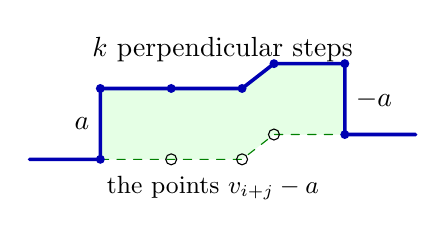
\begin{tikzpicture}[scale=0.9,line width=1.3pt,line cap=round,x={(1cm,0cm)},y={(0.45cm,0.35cm)},z={(0cm,1cm)}]
  \fill[green!10] (0,0,0) -- (0,0,1) -- (1,0,1) -- (2,0,1) -- (2,1,1) -- (3,1,1) -- (3,1,0) -- (2,1,0) -- (2,0,0) -- (1,0,0) -- cycle;
  \draw[thin,dashed,green!50!black] (0,0,0) -- (1,0,0) -- (2,0,0) -- (2,1,0) -- (3,1,0);
  \draw[blue!70!black] (-1,0,0) -- (0,0,0) -- (0,0,1) -- (1,0,1) -- (2,0,1) -- (2,1,1) -- (3,1,1) -- (3,1,0) -- (4,1,0);
  \foreach \p in {(0,0,0),(0,0,1),(1,0,1),(2,0,1),(2,1,1),(3,1,1),(3,1,0)} \fill[blue!70!black] \p circle (1.8pt);
  \foreach \p in {(1,0,0),(2,0,0),(2,1,0)} \draw[thin] \p circle (2.2pt);
  \node[left] at (0,0,0.5) {$a$};
  \node[right] at (3,1,0.5) {$-a$};
  \node[above] at (1.5,0.5,1.05) {$k$ perpendicular steps};
  \node[below] at (1.5,0.2,-0.15) {\small the points $v_{i+j}-a$};
\end{tikzpicture}
\caption{A curtain: a step $a$, then $k$ perpendicular steps, then $-a$.  If none of the circled
points below its interior is a vertex, the shaded curtain can be pushed down: $k-1$ corner flips and
one U-turn removal shorten the polygon by two.  So in a shortest polygon some circled point is always
a vertex (condition C6).}
\label{fig:curtain}
\end{figure}

\paragraph*{Pushing down.}  Among all shortest polygons of type $5_2$ or $5_2^*$, first permute the
axes so that the polygon has at most as many $z$-steps as $y$-steps and at most as many $y$-steps as
$x$-steps.  Then choose one that minimises the total height
$\Psi=\sum_i (z(v_i)-z_{\min})$, and among those the total depth $\Psi_2=\sum_i(y(v_i)-y_{\min})$.
Now look at a corner where the polygon goes up and then horizontally.  If the fourth corner of its
square were free, flipping it would lower one vertex by one unit and decrease $\Psi$; so in our chosen
polygon that point is a vertex.  The same holds for the three other corner patterns that a flip could
push downwards (or towards $-y$).

\paragraph*{Canonical position.}  Finally translate the polygon so that its least vertex in the order
$(z,y,x)$ is the origin, start the word there, and pick the direction of traversal by a fixed rule.

\begin{theorem}[Normal form; Lean: \lean{exists\_survivor}]\label{thm:normal}
If a polygon of type $5_2$ or $5_2^*$ has at most $34$ steps, then some polygon word $w$ of type
$5_2$ or $5_2^*$ with $|w|\le34$ is a unit square or satisfies
\begin{description}
\item[C1--C2] $w$ is a polygon word;
\item[C3] every vertex other than $v_0$ is greater than $v_0=0$ in the order $(z,y,x)$;
\item[C4] the first letter is smaller than the reverse of the last, in the order $\word{e}<\word{n}<\word{u}$;
\item[C5] $\#z\le\#y\le\#x$ letters;
\item[C6] (curtains) for every step $a$ followed by $k\ge1$ perpendicular steps and then $-a$, some
point $v_{i+j}-a$, $2\le j\le k$, is a vertex;
\item[C7] (corners) at every vertex $v_i$, $1\le i<n$, whose corner a flip would move down (or towards
$-y$ at constant height), the fourth corner of the square is a vertex.
\end{description}
\end{theorem}

Unit squares are unknots, so they are excluded by the colouring test.  The point of
\cref{thm:normal} is that C1--C7 are \emph{local} conditions that a search can test on partial
walks, long before the walk closes.

%=====================================================================================================
\section{Stage two: the search}\label{sec:search}

The search builds walks from the origin one step at a time, trying the six letters in a fixed order,
and backtracks as soon as a test shows that the partial walk cannot be completed to a closed walk of
length $n$ satisfying C1--C7.

The key device is the \emph{obligation}.  When the walk completes a curtain (C6) or turns a corner
covered by C7, the condition does not fail or succeed yet: it says that one of a few specific lattice
points must \emph{eventually} be a vertex.  The search records these points as a pending obligation.
An obligation is met when the walk later visits one of its points, and every pending obligation
constrains the rest of the walk.  The tests are:

\begin{description}
\item[Self-avoidance and position.] The next vertex is new, is greater than the origin in
$(z,y,x)$ order (C3), and is within distance $R-1$ of the origin, where $R$ is the number of steps
left.
\item[No U-turns.] A step may not reverse the step two places before it (C6 with $k=1$).
\item[Axis counts.] The counts so far must still be completable to $\#z\le\#y\le\#x$ (C5).
\item[Reach.] Every pending obligation has a point $s$ that can be reached and left in time: the head
can walk to $s$ and from $s$ back to the origin within the remaining steps, and $s$ has two
neighbours that are free, the head, or the origin.
\item[Span.] The rest of the walk must visit all single-point obligations; on each axis its
coordinate must sweep the interval spanned by them, the head and the origin, which costs at least
$\min(a_1,a_2)$ steps on that axis; the sum over the three axes must not exceed $R-1$.
\item[Closing.] At the last step: the walk closes at the origin, no obligation is pending, the
curtains that wrap around the origin are satisfied, and C4 and C5 hold.
\end{description}

\begin{theorem}[Completeness; Lean: \lean{search\_complete}]\label{thm:complete}
Every word $w$ with $|w|\le 34$ that satisfies C1--C7 is returned by the search.
\end{theorem}

The heart of the proof is an invariant: \emph{every pending obligation contains a point that is a
later vertex of $w$}.  A new obligation is created from an instance of C6 or C7 for $w$, which
names a vertex of $w$; if that vertex were already visited, the obligation would have been met at
once.  Given the invariant, the reach test passes along $w$ because $w$ itself walks to that vertex
and home again in time, and the span test passes because $w$'s remaining steps visit all those
vertices.  The other tests are direct consequences of C1--C7.

\begin{table}[t]
\centering
\caption{The proof runs.  For each length $n$: the number of parts the run was split into, the parts
accepted (\cref{sec:engineering}), the search nodes summed over the parts, and the number of distinct
words returned.  Every returned word passed the colouring test.  For split runs the node sums count
the shallow part of the tree once per part.  No polygon of length $\le 22$ satisfies C1--C7.}
\label{tab:runs}
\begin{tabular}{rrrrr}
\toprule
$n$ & parts & accepted & nodes & words \\
\midrule
4 & 1 & 1 & \num{9} & \num{0} \\
6 & 1 & 1 & \num{41} & \num{0} \\
8 & 1 & 1 & \num{211} & \num{0} \\
10 & 1 & 1 & \num{1189} & \num{0} \\
12 & 1 & 1 & \num{6548} & \num{0} \\
14 & 1 & 1 & \num{33635} & \num{0} \\
16 & 1 & 1 & \num{183243} & \num{0} \\
18 & 1 & 1 & \num{996110} & \num{0} \\
20 & 1 & 1 & \num{5378764} & \num{0} \\
22 & 1 & 1 & \num{30829429} & \num{0} \\
24 & 1 & 1 & \num{181235380} & \num{56} \\
26 & 1 & 1 & \num{1078116768} & \num{168} \\
28 & 2 & 2 & \num{6772583100} & \num{712} \\
30 & 64 & 64 & \num{43638057581} & \num{2782} \\
32 & 256 & 256 & \num{283692993804} & \num{7212} \\
34 & 1024 & 1024 & \num{1929898505964} & \num{22070} \\
\bottomrule
\end{tabular}

\end{table}

\Cref{tab:runs} shows the size of the search; \cref{fig:growth} shows its growth, about a factor of
\NGrowth{} per step of two.  The resulting set: \textbf{\NWords{} words} of lengths 24 to 34.

\begin{figure}[t]
\centering
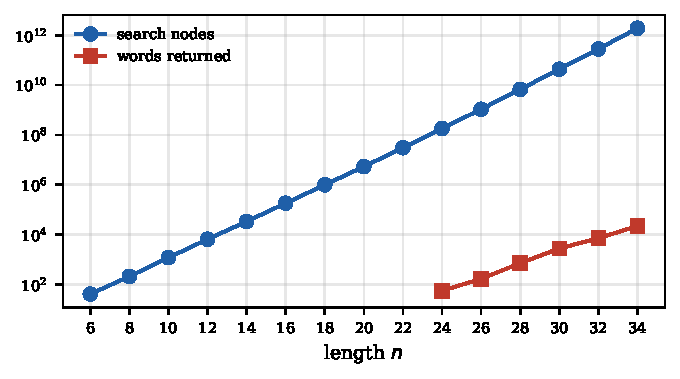
\includegraphics[width=0.7\linewidth]{figs/growth.pdf}
\caption{Search nodes and returned words per length (logarithmic scale).}
\label{fig:growth}
\end{figure}

%=====================================================================================================
\section{Stage three: ruling out $5_2$ with Fox colourings}\label{sec:colour}

Each returned word is a lattice polygon of some knot type.  An earlier, unverified identification
by Reidemeister simplification finds only unknots, trefoils, figure-eight knots and cinquefoils among
them.  But we do not need to know \emph{which} knot each word is; we only need to know that it is not
$5_2$.  For this the Fox $7$-colourings suffice, and they come with a certificate that is trivial to
check.

\begin{theorem}[Lean hypothesis \lean{TopHyp}; proved from the Wirtinger presentation]\label{thm:fox}
The number of Fox $7$-colourings of a regular diagram depends only on the knot group, and is the same
for a knot and its mirror image.
\end{theorem}

\begin{proof}
Let $D_7$ act on $\Z/7$ by $t\mapsto\pm t+c$; its reflections $r_a(t)=2a-t$ are distinct and satisfy
$r_br_ar_b=r_{2b-a}$.  Let $\sigma:D_7\to\Z/2$ detect reflections, and let $\alpha:G\to\Z/2$ be the
unique surjection of the knot group $G=\pi_1(\R^3\setminus K)$, the abelianisation $G\to\Z$ reduced
mod 2.  The set of homomorphisms $\varphi:G\to D_7$ with $\sigma\circ\varphi=\alpha$ depends only on
$G$.  In the Wirtinger presentation~\cite{BZ,Rol76} read from a regular diagram, every generator
(arc) maps to $1\in\Z$, so such a $\varphi$ sends every arc to a reflection $r_{a_i}$; and the
relation $x_{\mathrm{out}}=x_{\mathrm{over}}^{\pm1}x_{\mathrm{in}}x_{\mathrm{over}}^{\mp1}$ holds
exactly when $a_{\mathrm{out}}=2a_{\mathrm{over}}-a_{\mathrm{in}}$, which is the Fox equation.  So
these homomorphisms are exactly the Fox colourings.
\end{proof}

\begin{lemma}\label{lem:fiftytwo}
Every regular diagram of $5_2$ or $5_2^*$ has a non-constant Fox $7$-colouring; there are $49$
colourings in all.
\end{lemma}

\begin{proof}
In the standard diagram, with PD code
\[ [1,5,2,4],\ [3,9,4,8],\ [5,1,6,10],\ [7,3,8,2],\ [9,7,10,6], \]
the arcs are $A=\{2,3\}$, $B=\{4,5\}$, $C=\{6,7\}$, $D=\{8,9\}$, $E=\{10,1\}$ and the equations are
$2B=E+A$, $2D=A+B$, $2E=B+C$, $2A=C+D$, $2C=D+E$.  Their solutions mod 7 are
$a(1,1,1,1,1)+b(0,1,3,4,2)$: $49$ colourings.  By \cref{thm:fox} the same holds for every diagram.
(For the 36-step polygon itself the colouring $(0,1,3,4,2)$ of \cref{fig:polygon} is checked by the
Lean kernel.)
\end{proof}

\paragraph*{Certificates.}  For a returned word, the program picks a projection direction from a
short fixed list for which the projection is regular, builds the $c\times c$ Fox matrix $F$ mod 7,
and finds by Gaussian elimination a matrix $L$ with $c-1$ rows such that row $k$ of $LF$ is
$e_k-e_0$.  It then \emph{checks} $LF\equiv E$.  If $x$ is any colouring then $Fx\equiv0$, so
$(LF)x\equiv0$, so $x_k\equiv x_0$ for all $k$: only constant colourings.  The elimination is
untrusted; only the multiplication check matters, and its soundness is a Lean theorem
(\lean{colorCheck\_sound}).

The resulting set: \textbf{0 words} that could be $5_2$.  By \cref{thm:normal,thm:complete}, no
polygon of type $5_2$ has at most 34 steps.

%=====================================================================================================
\section{The upper bound}\label{sec:upper}

The word
\[ w_{36}=\word{eeennuwwwwssseennwuueedddnnuuswsswdd} \]
is a polygon word of length 36.  Projected along $(1,-19,40)$---or, more legibly, along $(5,-5,11)$
as in \cref{fig:polygon}---it has a regular diagram with five crossings whose PD code is a relabelling
of the mirror of the standard $5_2$ code.  This comparison is kernel-checked in Lean
(\lean{w52\_pd}), together with controls (the code of $5_1$ does not match; without the mirror
operation, the chiral knots $3_1$, $5_1$, $5_2$ are not equivalent to their mirrors while $4_1$ is).
A PD code is a rotation system of the diagram's 4-valent plane graph, so equal codes give diagrams that
differ by a homeomorphism of the sphere, and hence equivalent knots~\cite{MT01,Kne26,BZ}.
Independently, SnapPy~\cite{SnapPy} identifies the complement as the census manifold
\texttt{m015}, the complement of $5_2$.

In fact the proof never needs the name ``$5_2$'' until this point: we may \emph{define}
$\Kft$ as the knot type of $|w_{36}|$, and then both bounds for $\Kft$ use only the
diagram of $w_{36}$ itself; the PD comparison is needed only to say that $\Kft$ is the
knot that the tables call $5_2$.

%=====================================================================================================
\section{The formalisation}\label{sec:lean}

The Lean development (plain Lean~4.25, no Mathlib, about \num{4500} lines) proves one theorem:

\begin{lstlisting}
theorem no_short (T : List Nat → Prop) (hT : KnotClass T) (hTop : TopHyp T)
    (hComp : CompCert) : ∀ w, T w → 36 ≤ w.length
\end{lstlisting}

Here $T$ is any class of words.  \lean{KnotClass T} says that $T$ consists of polygon words and is
closed under rotation and reversal of the word, under the 48 lattice symmetries, under valid corner
flips and under U-turn removals; \lean{TopHyp T} says that every regular diagram of a member of $T$
has a non-constant Fox $7$-colouring; and \lean{CompCert} is the finite computation.  Applied to
$T=\{w : |w|\text{ is of type }5_2\text{ or }5_2^*\}$, the first two hypotheses are the classical
facts of \cref{lem:moves} and \cref{thm:fox,lem:fiftytwo}.  \Cref{fig:arch} shows how the proof
fits together.

\begin{figure}[t]
\centering
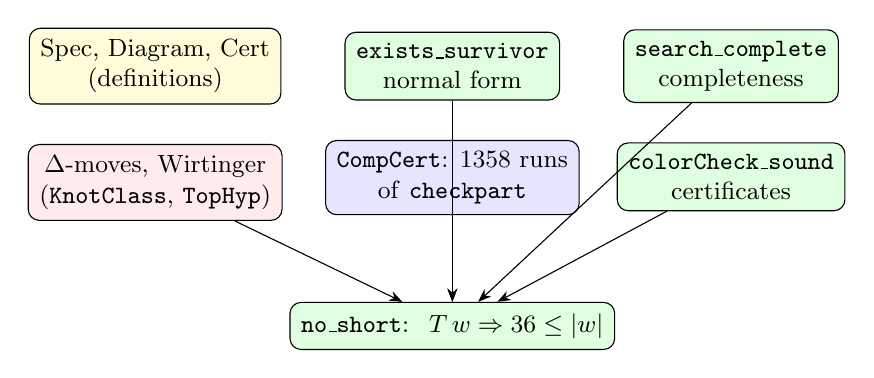
\begin{tikzpicture}[node distance=5mm and 8mm, box/.style={draw,rounded corners,align=center,font=\small,inner sep=4pt},
  stmt/.style={box,fill=yellow!15}, thm/.style={box,fill=green!12}, comp/.style={box,fill=blue!10}, cls/.style={box,fill=red!8}]
  \node[stmt] (spec) {Spec, Diagram, Cert\\(definitions)};
  \node[thm, right=of spec] (nf) {\lean{exists\_survivor}\\normal form};
  \node[thm, right=of nf] (sc) {\lean{search\_complete}\\completeness};
  \node[thm, below=of sc] (cc) {\lean{colorCheck\_sound}\\certificates};
  \node[comp, below=of nf] (cp) {\lean{CompCert}: 1358 runs\\of \lean{checkpart}};
  \node[cls, below=of spec] (cl) {$\Delta$-moves, Wirtinger\\(\lean{KnotClass}, \lean{TopHyp})};
  \node[thm, below=11mm of cp, minimum width=40mm] (main) {\lean{no\_short}: \ $T\,w \Rightarrow 36\le|w|$};
  \foreach \a in {nf,sc,cc,cp,cl} \draw[-{Stealth}] (\a) -- (main);
\end{tikzpicture}
\caption{Structure of the proof.  Green: kernel-checked theorems.  Yellow: the statement.  Red:
classical knot theory, proved in the text.  Blue: the computation.}
\label{fig:arch}
\end{figure}

\paragraph*{The statement.}  A reader who wants to check the theorem must read the definitions
(polygon words, C1--C7, the moves, regular diagrams and Fox equations, and \lean{CompCert}) and the
statement of \lean{no\_short}.  Everything else is checked by the kernel.  \lean{\#print axioms}
reports only \lean{propext}, \lean{Classical.choice} and \lean{Quot.sound}; the sources contain no
\lean{sorry}, \lean{native\_decide}, \lean{implemented\_by} or
\lean{extern}, and a GitHub workflow
rebuilds everything from a clean checkout and prints the axioms.

\paragraph*{The program is the proof object.}  \Cref{thm:complete} is proved about the very program
that was run.  The search is written in a functional style that the kernel can reason about---walk
data in immutable lists, explicit structural recursion on the remaining steps---while keeping a
single mutable occupancy array, which the compiler updates in place.  It is a line-by-line equivalent
of an independent C\texttt{++} program and visits exactly the same number of nodes
(\cref{sec:cross}).

\paragraph*{A bug that only the proof could find.}  An early version of the Lean search looked up
the wrong vertex for the corner test C7: an off-by-one index into the reversed position list.  The
program still ran, and returned the same words as the C\texttt{++} program on every length we tried,
but it tested C7 at the wrong point, which in principle can discard valid walks.  It was caught
because the node counts differed from the C\texttt{++} program; a completeness proof would not have
gone through.  This is the kind of error that cross-checking outputs alone does not exclude.

%=====================================================================================================
\section{The computation}\label{sec:engineering}

By a one-line Lean lemma, \lean{CompCert} is equivalent to the truth of \num{1358} closed Boolean
terms $\mathtt{checkPart}\ n\ r$: for each even $n\le34$ and each part $r$ of a fixed split, run the
search for length $n$ restricted to part $r$ and check every returned word.  The executable
\texttt{checkpart} evaluates exactly this term, prints the words and a final line
\texttt{RESULT \dots\ ok=true}, and exits with status $0$ if and only if the term is true.

\paragraph*{Where it ran.}  The total is about \NNodes{} search nodes.  Lengths up to 30, and
half of the parts of length 32, ran in a 4-core container; the other half of length 32 and all 1024
parts of length 34 ran on GitHub Actions, which offers twenty free 4-core runners at a time for
public repositories.  At about $5\times10^5$ nodes per second per core, a part of length 34 took
between 40 and 90 minutes for most parts (median one hour); length 34 used about 1060 core-hours,
roughly half a day of wall time on the free runners.

\paragraph*{Provenance.}  A part is accepted only if its log records exit status $0$, its output ends
with the \texttt{RESULT} line for that part with the right number of words before it, the output's
SHA-256 matches the logged one, and the program was built from sources identical to the current
ones: for GitHub runs, a clean checkout of the logged commit, with the output files committed back
by the workflow's bot account in a commit naming the run; for local runs, a hash of the sources computed before the build and re-checked after
every part.  The output of each part is deterministic, so anyone can re-run any part and compare
hashes; we did so for a random sample of the GitHub parts.

\paragraph*{What is trusted.}  The compiled program evaluated the \num{1358} Booleans correctly: this
rests on the Lean compiler, its C back end, the runtime and the hardware---the usual trust model for
verified computations too large for the kernel.  It is backed by the independent C\texttt{++} program
(\cref{sec:cross}).

%=====================================================================================================
\section{Independent cross-checks}\label{sec:cross}

None of the following is needed for the proof; each tests it.
\begin{itemize}
\item \textbf{A second implementation.}  The C\texttt{++} enumerator in its cross-check mode
implements the same algorithm independently; for every length it returns the same set of words, and
for unsplit runs ($n\le26$) exactly the same number of nodes.
\item \textbf{Independent re-implementations of the definitions.}  A Python implementation of the
projection and colouring count finds exactly $7$ colourings for every returned word, and a Python
implementation of C1--C7 written by the referee from the Lean definitions alone accepts every
returned word.
\item \textbf{Known censuses.}  The flip-and-symmetry closure of the 50 trefoils returned at length 24
is the full set of 3328 shortest trefoil polygons known from~\cite{JvRR11}, and the earlier faster
runs reproduced the published numbers of shortest $4_1$ (3648) and $5_1$ (6672) polygons in the same
way.  A missing branch of the search would show up as a missing flip class.
\item \textbf{Adversarial review.}  The informal proof and the Lean sources were reviewed in two
rounds by an adversarial referee, who tested completeness on the trefoil census and the colouring
hypothesis on \num{12750} diagrams of sixty independently generated $5_2$ polygons.
\end{itemize}

%=====================================================================================================
\section{Discussion}\label{sec:discussion}

The value $\Len(5_2)=36$ is the first exact minimal lattice length for a knot beyond the three known
before, and the first with a fully formal proof.  The method extends.  The faster, unverified version
of the search (with the plane-crossing lemma, valid for prime knots, and a computer-checked arc
lemma for composites) has been run to length 36, where it finds only the unknot, $3_1$, $4_1$, $5_1$
and $5_2$; this indicates that every other knot needs at least 38 steps.  Making that statement
formal needs the arc lemma and the plane-crossing lemma in Lean, the second of which uses the prime
decomposition of knots.  Reaching length 40---which would settle $\Len(6_1)$, $\Len(6_2)$,
$\Len(6_3)$ and $\Len(3_1\#3_1)$, all believed to be 40---needs roughly $50$ times the present
computation, or a smarter normal form.

\subparagraph*{Acknowledgements.}  The programs, the Lean proofs and much of the text were developed
with the help of AI coding agents (Claude, Anthropic), including the adversarial review rounds; all
claims are checked as described above.

\bibliography{len52}

\end{document}
